\selectlanguage{hebrew}
\section{בסיס}
\label{sec:ch02}

מחקר מערכת אלגוריתם ניתוח תוצאות שיטה מודל פתרון חישן נתון עיבוד מדידה הערכה ביצוע ניסוי בדיקה תוצאה מסקנה מבנה ארכיטקטורה תכנון יישום פיתוח הדמיה מיפוי ניווט מיקום זיהוי סיווג אומדן גישה מסגרת כלי תהליך שלב מרכיב רכיב מודול מנגנון ביצועים שיפור מחקר מערכת אלגוריתם ניתוח תוצאות שיטה מודל פתרון חישן נתון עיבוד מדידה הערכה ביצוע ניסוי בדיקה תוצאה מסקנה מבנה ארכיטקטורה תכנון יישום פיתוח הדמיה מיפוי ניווט מיקום זיהוי סיווג אומדן גישה מסגרת כלי תהליך שלב מרכיב רכיב מודול מנגנון ביצועים שיפור מחקר מערכת אלגוריתם ניתוח תוצאות שיטה מודל פתרון חישן נתון עיבוד מדידה הערכה ביצוע ניסוי בדיקה תוצאה מסקנה מבנה ארכיטקטורה תכנון יישום פיתוח הדמיה מיפוי ניווט מיקום זיהוי סיווג אומדן גישה מסגרת כלי תהליך שלב מרכיב רכיב מודול מנגנון ביצועים שיפור מחקר מערכת אלגוריתם ניתוח תוצאות שיטה מודל פתרון חישן נתון עיבוד מדידה הערכה ביצוע ניסוי בדיקה תוצאה מסקנה מבנה ארכיטקטורה תכנון יישום פיתוח הדמיה מיפוי ניווט מיקום זיהוי סיווג אומדן גישה מסגרת כלי תהליך שלב מרכיב רכיב מודול מנגנון

\subsection{בסיס 1}
\label{sub:ch02_1}
מחקר מערכת אלגוריתם ניתוח תוצאות שיטה מודל פתרון חישן נתון עיבוד מדידה הערכה ביצוע ניסוי בדיקה תוצאה מסקנה מבנה ארכיטקטורה תכנון יישום פיתוח הדמיה מיפוי ניווט מיקום זיהוי סיווג אומדן גישה מסגרת כלי תהליך שלב מרכיב רכיב מודול מנגנון ביצועים שיפור מחקר מערכת אלגוריתם ניתוח תוצאות שיטה מודל פתרון חישן נתון עיבוד מדידה הערכה ביצוע ניסוי בדיקה תוצאה מסקנה מבנה ארכיטקטורה תכנון יישום פיתוח הדמיה מיפוי ניווט מיקום זיהוי סיווג אומדן גישה מסגרת כלי תהליך שלב מרכיב רכיב מודול מנגנון ביצועים שיפור מחקר מערכת אלגוריתם ניתוח תוצאות שיטה מודל פתרון חישן נתון עיבוד מדידה הערכה ביצוע ניסוי בדיקה תוצאה מסקנה מבנה ארכיטקטורה תכנון יישום פיתוח הדמיה מיפוי ניווט מיקום זיהוי סיווג אומדן גישה מסגרת כלי תהליך שלב מרכיב רכיב מודול מנגנון ביצועים שיפור מחקר מערכת אלגוריתם ניתוח תוצאות שיטה מודל פתרון חישן נתון עיבוד מדידה הערכה ביצוע ניסוי בדיקה תוצאה מסקנה מבנה ארכיטקטורה תכנון יישום פיתוח הדמיה מיפוי ניווט מיקום זיהוי סיווג אומדן גישה מסגרת כלי תהליך שלב מרכיב רכיב מודול מנגנון

\begin{equation}
    x_{k+1} = A_{k} x_k + B u_{k} + w_{1}
    \label{eq:ch02_1}
\end{equation}
מחקר מערכת אלגוריתם ניתוח תוצאות שיטה מודל פתרון חישן נתון עיבוד מדידה הערכה ביצוע ניסוי

\subsection{בסיס 2}
\label{sub:ch02_2}
מחקר מערכת אלגוריתם ניתוח תוצאות שיטה מודל פתרון חישן נתון עיבוד מדידה הערכה ביצוע ניסוי בדיקה תוצאה מסקנה מבנה ארכיטקטורה תכנון יישום פיתוח הדמיה מיפוי ניווט מיקום זיהוי סיווג אומדן גישה מסגרת כלי תהליך שלב מרכיב רכיב מודול מנגנון ביצועים שיפור מחקר מערכת אלגוריתם ניתוח תוצאות שיטה מודל פתרון חישן נתון עיבוד מדידה הערכה ביצוע ניסוי בדיקה תוצאה מסקנה מבנה ארכיטקטורה תכנון יישום פיתוח הדמיה מיפוי ניווט מיקום זיהוי סיווג אומדן גישה מסגרת כלי תהליך שלב מרכיב רכיב מודול מנגנון ביצועים שיפור מחקר מערכת אלגוריתם ניתוח תוצאות שיטה מודל פתרון חישן נתון עיבוד מדידה הערכה ביצוע ניסוי בדיקה תוצאה מסקנה מבנה ארכיטקטורה תכנון יישום פיתוח הדמיה מיפוי ניווט מיקום זיהוי סיווג אומדן גישה מסגרת כלי תהליך שלב מרכיב רכיב מודול מנגנון ביצועים שיפור מחקר מערכת אלגוריתם ניתוח תוצאות שיטה מודל פתרון חישן נתון עיבוד מדידה הערכה ביצוע ניסוי בדיקה תוצאה מסקנה מבנה ארכיטקטורה תכנון יישום פיתוח הדמיה מיפוי ניווט מיקום זיהוי סיווג אומדן גישה מסגרת כלי תהליך שלב מרכיב רכיב מודול מנגנון

\begin{equation}
    x_{k+2} = A_{k} x_k + B u_{k} + w_{2}
    \label{eq:ch02_2}
\end{equation}
מחקר מערכת אלגוריתם ניתוח תוצאות שיטה מודל פתרון חישן נתון עיבוד מדידה הערכה ביצוע ניסוי

\subsection{בסיס 3}
\label{sub:ch02_3}
מחקר מערכת אלגוריתם ניתוח תוצאות שיטה מודל פתרון חישן נתון עיבוד מדידה הערכה ביצוע ניסוי בדיקה תוצאה מסקנה מבנה ארכיטקטורה תכנון יישום פיתוח הדמיה מיפוי ניווט מיקום זיהוי סיווג אומדן גישה מסגרת כלי תהליך שלב מרכיב רכיב מודול מנגנון ביצועים שיפור מחקר מערכת אלגוריתם ניתוח תוצאות שיטה מודל פתרון חישן נתון עיבוד מדידה הערכה ביצוע ניסוי בדיקה תוצאה מסקנה מבנה ארכיטקטורה תכנון יישום פיתוח הדמיה מיפוי ניווט מיקום זיהוי סיווג אומדן גישה מסגרת כלי תהליך שלב מרכיב רכיב מודול מנגנון ביצועים שיפור מחקר מערכת אלגוריתם ניתוח תוצאות שיטה מודל פתרון חישן נתון עיבוד מדידה הערכה ביצוע ניסוי בדיקה תוצאה מסקנה מבנה ארכיטקטורה תכנון יישום פיתוח הדמיה מיפוי ניווט מיקום זיהוי סיווג אומדן גישה מסגרת כלי תהליך שלב מרכיב רכיב מודול מנגנון ביצועים שיפור מחקר מערכת אלגוריתם ניתוח תוצאות שיטה מודל פתרון חישן נתון עיבוד מדידה הערכה ביצוע ניסוי בדיקה תוצאה מסקנה מבנה ארכיטקטורה תכנון יישום פיתוח הדמיה מיפוי ניווט מיקום זיהוי סיווג אומדן גישה מסגרת כלי תהליך שלב מרכיב רכיב מודול מנגנון

\begin{equation}
    x_{k+3} = A_{k} x_k + B u_{k} + w_{3}
    \label{eq:ch02_3}
\end{equation}
מחקר מערכת אלגוריתם ניתוח תוצאות שיטה מודל פתרון חישן נתון עיבוד מדידה הערכה ביצוע ניסוי

\begin{figure}[htbp]
    \centering
    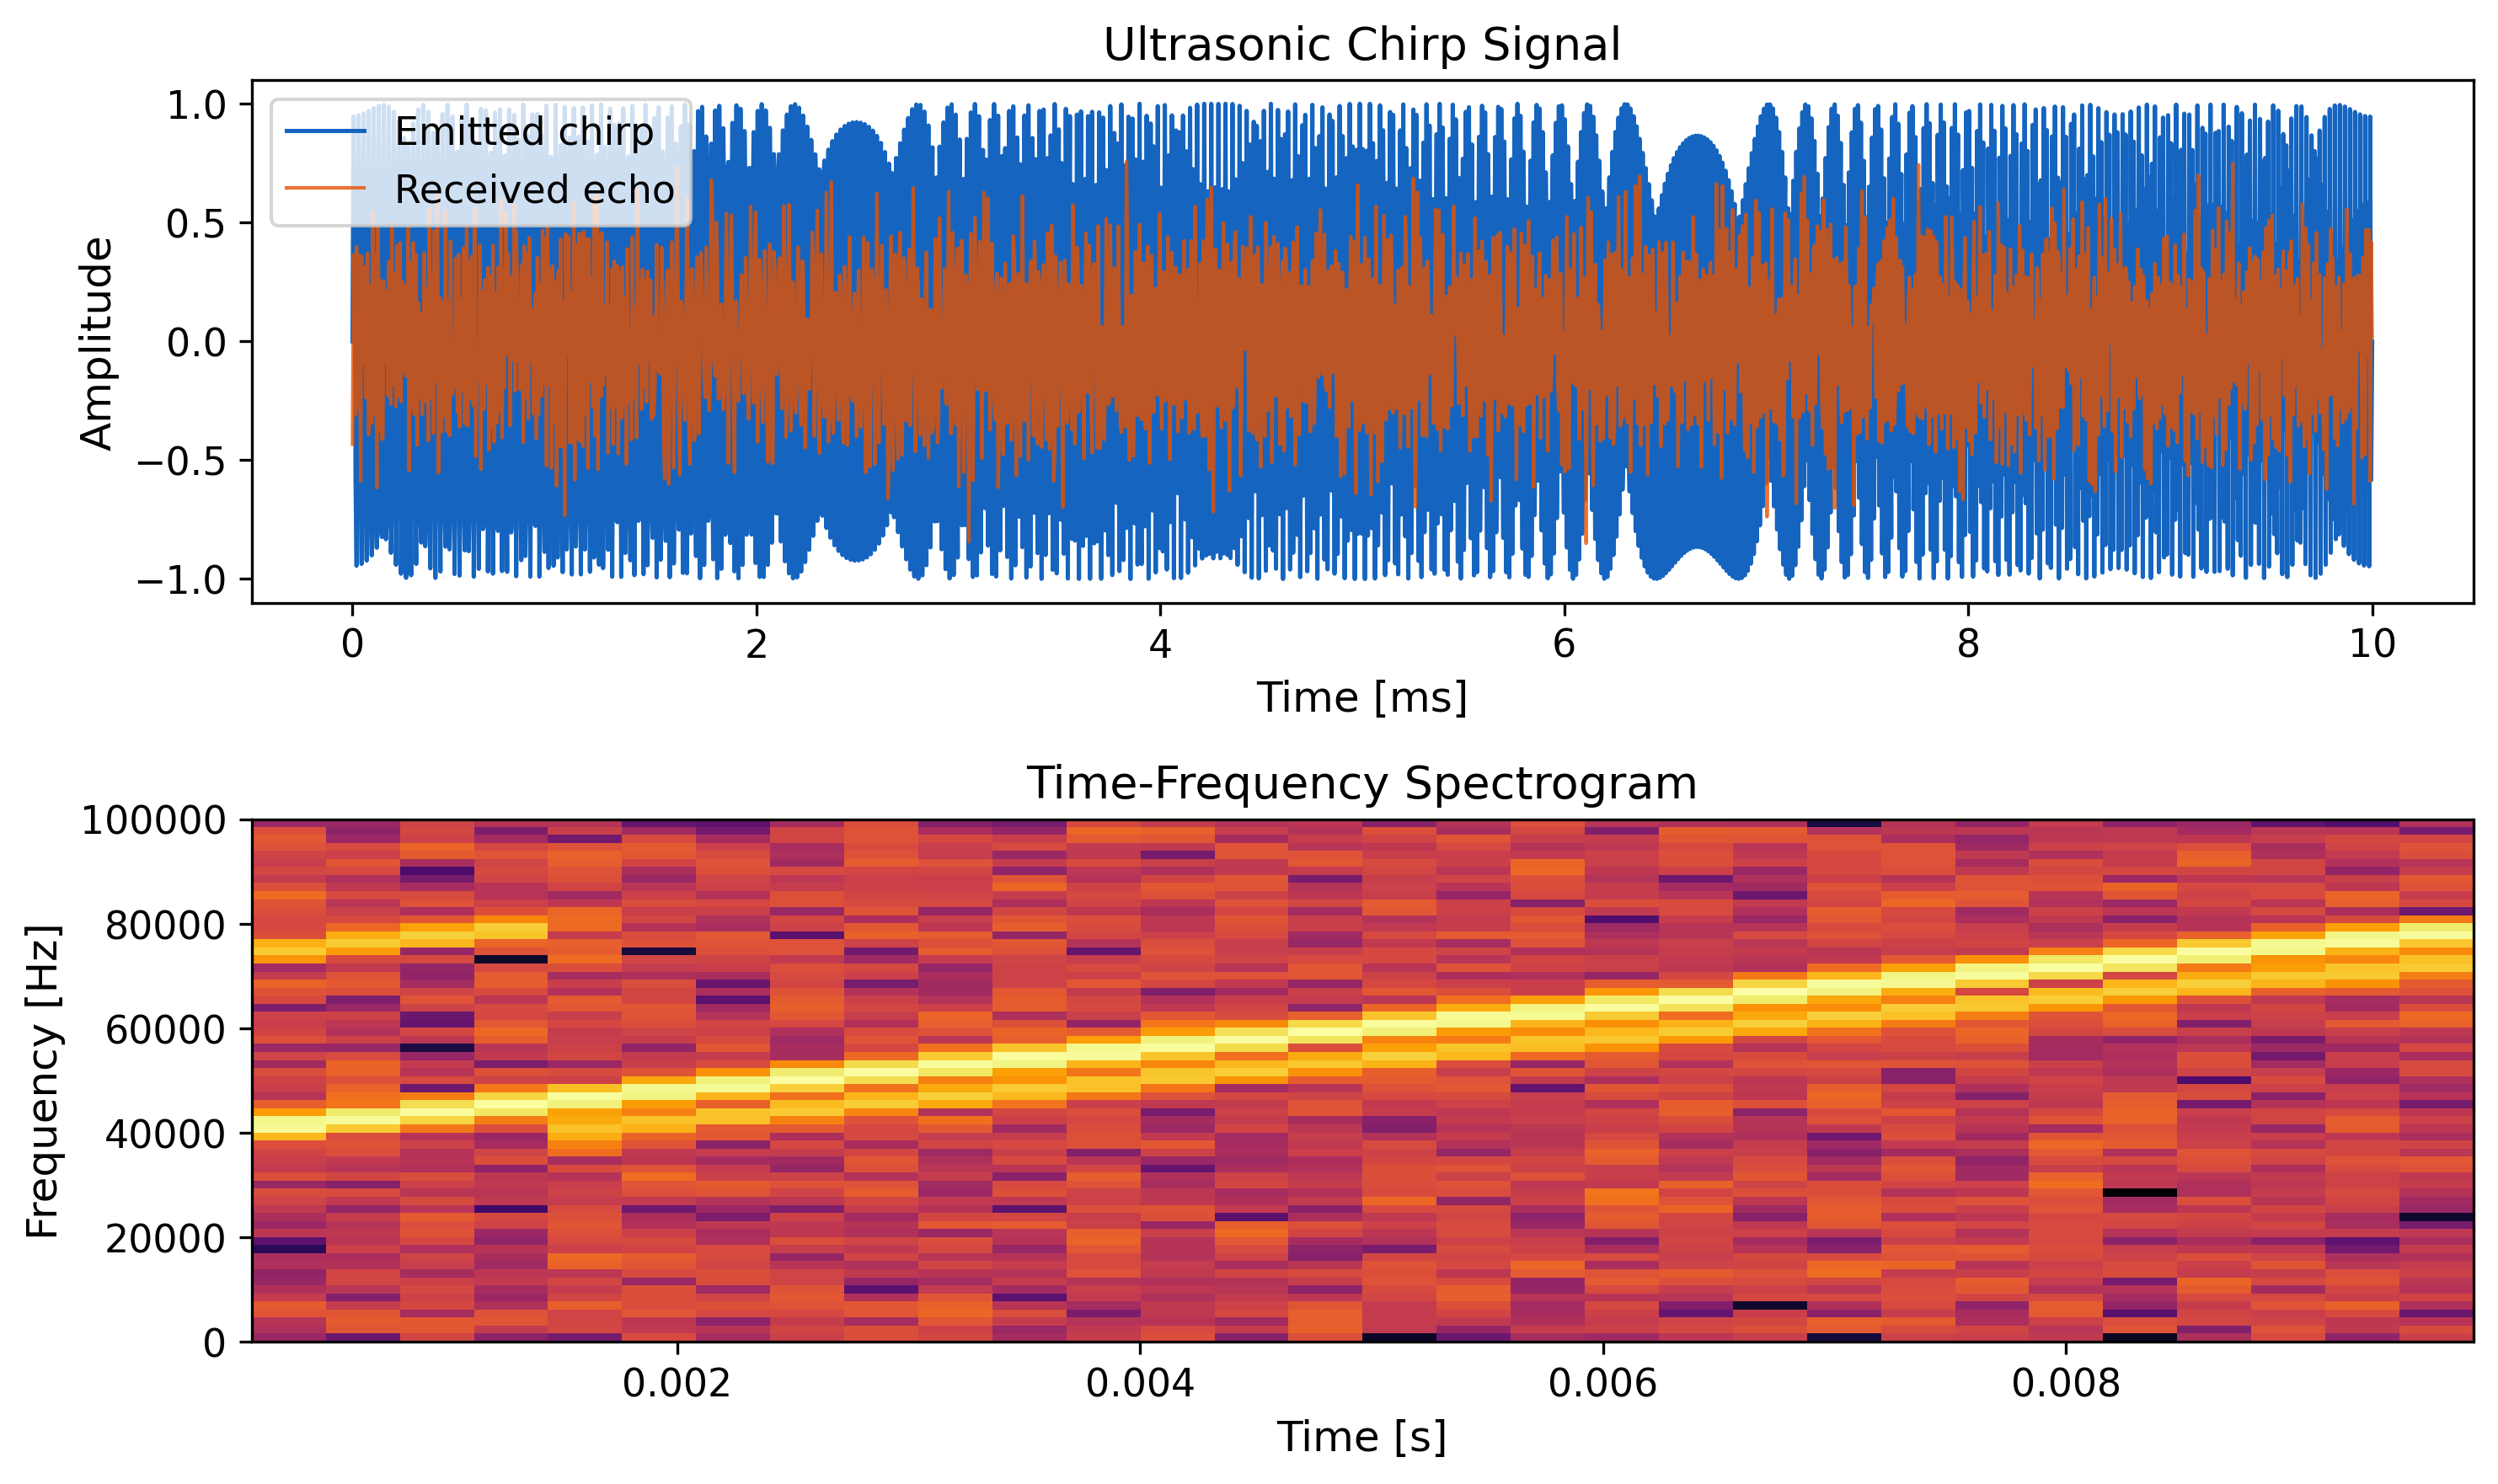
\includegraphics[width=0.9\columnwidth]{figures/fig_ch02_auto.png}
    \caption{Stub figure 1 : ch02}
    \label{fig:ch02_1}
\end{figure}

\en{See} \cite{Thrun2005}\cite{Kalman1960}.